%%%%%%%%%%%%%%%%%%%%%%%%%%%%%%%%%%%%%%%%%%%%%%%%%%%%%%%%%%%%%%%%%
% MUW Presentation
% LaTeX Template
% Version 1.0 (27/12/2016)
%
% License:
% CC BY-NC-SA 4.0 (http://creativecommons.org/licenses/by-nc-sa/3.0/)
%
% Created by:
% Nicolas Ballarini, CeMSIIS, Medical University of Vienna
% nicoballarini@gmail.com
% http://statistics.msi.meduniwien.ac.at/
%
% Customized for UAH by:
% David F. Barrero, Departamento de Automática, UAH
%%%%%%%%%%%%%%%%%%%%%%%%%%%%%%%%%%%%%%%%%%%%%%%%%%%%%%%%%%%%%%%%%

\documentclass[10pt,compress]{beamer} % Change 10pt to make fonts of a different size
\mode<presentation>

\usepackage[spanish]{babel}
\usepackage{fontspec}
\usepackage{tikz}
\usepackage{etoolbox}
\usepackage{xcolor}
\usepackage{xstring}
\usepackage{listings}
\usepackage{tikz}
\usetikzlibrary{matrix,chains,positioning,decorations.pathreplacing,arrows,shapes}

\usetheme{UAH}
\usecolortheme{UAH}
\setbeamertemplate{navigation symbols}{} 
\setbeamertemplate{caption}[numbered]

%%%%%%%%%%%%%%%%%%%%%%%%%%%%%%%%%%%%%%%%%%%%%%%%%%%%%%%%%%%%%%%%%
%% Presentation Info
\title[Input and output]{Input and output}
\author{\asignatura\\\carrera}
\institute{}
\date{Departamento de Automática}
%%%%%%%%%%%%%%%%%%%%%%%%%%%%%%%%%%%%%%%%%%%%%%%%%%%%%%%%%%%%%%%%%


%%%%%%%%%%%%%%%%%%%%%%%%%%%%%%%%%%%%%%%%%%%%%%%%%%%%%%%%%%%%%%%%%
%% Descomentar para habilitar barra de navegación superior
\setNavigation
%%%%%%%%%%%%%%%%%%%%%%%%%%%%%%%%%%%%%%%%%%%%%%%%%%%%%%%%%%%%%%%%%

%%%%%%%%%%%%%%%%%%%%%%%%%%%%%%%%%%%%%%%%%%%%%%%%%%%%%%%%%%%%%%%%%
%% Configuración de logotipos en portada
%% Opacidad de los logotipos
\newcommand{\opacidad}{1}
%% Descomentar para habilitar logotipo en pié de página de portada
\renewcommand{\logoUno}{Images/isg.png}
%% Descomentar para habilitar logotipo en pié de página de portada
%\renewcommand{\logoDos}{Images/CCLogo.png}
%% Descomentar para habilitar logotipo en pié de página de portada
%\renewcommand{\logoTres}{Images/ALogo.png}
%% Descomentar para habilitar logotipo en pié de página de portada
%\renewcommand{\logoCuatro}{Images/ELogo.png}
%%%%%%%%%%%%%%%%%%%%%%%%%%%%%%%%%%%%%%%%%%%%%%%%%%%%%%%%%%%%%%%%%

%%%%%%%%%%%%%%%%%%%%%%%%%%%%%%%%%%%%%%%%%%%%%%%%%%%%%%%%%%%%%%%%%
%% FOOTLINE
%% Comment/Uncomment the following blocks to modify the footline
%% content in the body slides. 


%% Option A: Title and institute
\footlineA
%% Option B: Author and institute
%\footlineB
%% Option C: Title, Author and institute
%\footlineC
%%%%%%%%%%%%%%%%%%%%%%%%%%%%%%%%%%%%%%%%%%%%%%%%%%%%%%%%%%%%%%%%%

\begin{document}

%%%%%%%%%%%%%%%%%%%%%%%%%%%%%%%%%%%%%%%%%%%%%%%%%%%%%%%%%%%%%%%%%
% Use this block for a blue title slide with modified footline
{\titlepageBlue
    \begin{frame}
        \titlepage
    \end{frame}
}

\begin{frame}[plain]{}
	\begin{block}{Objectives}
		\begin{enumerate}
		\item Being able to apply output formatting methods in Python.
		\item Being able to manipulate files in Python.
		\item Being able to understand the usefulness of Python serialization (\textit{pickles}).
		\end{enumerate}
	\end{block}
\end{frame}

{
\disableNavigation{white}
\begin{frame}[shrink]{Table of Contents}
 \frametitle{Table of Contents}
 \tableofcontents
  % You might wish to add the option [pausesections]
\end{frame}
}

\section{Input and output}

\subsection{Introduction}
\begin{frame}[fragile]{Input and output}{Introduction}
    \begin{columns}
 	   \column{.60\textwidth}
			\textbf{Input/output}: How the program can read and export data.
 	   \column{.40\textwidth}
  		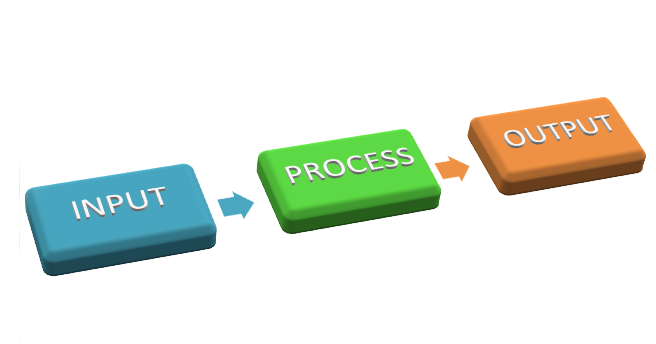
\includegraphics[width=\textwidth]{figs/io.png}\\
		%\centering \tiny{Source: \url{http://www.justprograming.com/wp-content/uploads/2014/05/output-transformation.png}}
	\end{columns}

    \begin{columns}
 	   \column{.60\textwidth}
	\begin{itemize}
		\item So far, we have used two methods to output information:
			\begin{itemize}
			\item Expressions statements and the \texttt{print()} function.
			\end{itemize}
		\item A third method: Standard input and output.\\
	\end{itemize}
    \column{.40\textwidth}
  			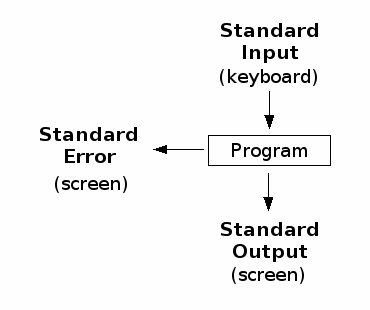
\includegraphics[width=\textwidth]{figs/InputOutput.png}\\
			\centering \tiny{Source: \url{http://labor-liber.org/en/gnu-linux/introduction/input\_output}}
	\end{columns}
\end{frame}

\subsection{Input and Output interactive}


\begin{frame}[fragile]{I/O interactive}{Data input}
Enter data  by keyboard  (version 2.X)
%(version 2.X works, in my 3.X does not):
\begin{verbatim}
>>> x = raw_input('Introduzca un numero:   ')
64.5
>>> y = float(x) ** 2
\end{verbatim}	
	Enter data  by keyboard  (version 3.X)
\begin{verbatim}	
>>> x = input('Introduzca un numero:   ')
64.5
>>> y = x ** 2
\end{verbatim}
\end{frame}

\begin{frame}[fragile]{I/O interactive}{Data output (I)}
Print \textbf{not formatted} data (version 2.X):\\
Needs () for version 3.X
\begin{verbatim}
>>> print 'message', var1, var2, ..., vark
\end{verbatim}
% las variables separadas por un blanco
Prints on the screen: \alert{message var1 var2 vark}
\begin{verbatim}
>>> name = 'John'
>>> age = 37
>>> print 'Name, age= ', name, age
Name, age= John 37
>>> print 'Name = ', name, ' age = ', age
Name = John age = 37
\end{verbatim}
\end{frame}

\begin{frame}[fragile]{I/O interactive}{Data output (II)}
Print \textbf{formatted} data (version 2.X):
\begin{verbatim}
>>> print 'msg1 = %type1 msg2 = %type2' % (var1, var2)
\end{verbatim}
where \texttt{type1} and   \texttt{type2} indicate how to represent the variable:\\	
\hspace{0.5cm}\%i and \%d: integer number.\\
\hspace{0.5cm}\%f: real number with decimal point.\\
\hspace{0.5cm}\%e: real number in exponential format.\\
\hspace{0.5cm}\%g: remove not significant zeros.\\
\hspace{0.5cm}\%s: string.\\
\footnotesize{\begin{verbatim}
>>> name = 'John'
>>> daybal = 55.5
>>> print '%s earns per month %6.2f euros' % (name,  daybal *30.)
John earns per month 1515.00 euros
\end{verbatim}
}
\end{frame}



\section{Fancier output formatting}

\subsection{Methods}
\begin{frame}{Methods}{Custom output}
	\begin{itemize}
		\item Two methods to create custom output:
			\begin{itemize}
			\item String manipulation.
			\item The \texttt{str.format()} method.
			\end{itemize}
		\item \textbf{Convert values to strings}:
			\begin{itemize}
			\item \texttt{str()}: Human-readable format.
			\item \texttt{repr()}: Interpreter-readable format.
			\item Both, are quite similar. But, strings have two representations:\\
			\footnotesize{\texttt{$>>>$ str1 = ``Hellow$\backslash$n"}}\\
			\textcolor{green}{\footnotesize{\texttt{$>>>$ str(str1)}}\\
			\footnotesize{\texttt{'Hellow$\backslash$n'}}}\\
			\alert{\footnotesize{\texttt{$>>>$ repr(str1)}}}\\
			\alert{\footnotesize{\texttt{``'Hellow$\backslash\backslash$n'"}}}\\
			\textcolor{blue}{\footnotesize{\texttt{$>>>$ repr([234, ('hellow', 'bye')])}}\\
			\footnotesize{\texttt{"[234, ('hellow', 'bye')]"}}\\
			\footnotesize{\texttt{$>>>$ str([234, ('hellow', 'bye')])}}\\
			\footnotesize{\texttt{"[234, ('hellow', 'bye')]"}}}\\	
			% por eso, cuando se imprime con print, con repr, la cadena se muestra con el \n que no se interpreta.
			% >>> print(repr(str1))
		%'Hellow\n'
		%>>> print(str(str1))
		%Hellow
			\end{itemize}
			
			
	\end{itemize}
\end{frame}

\subsection{Examples of fancy output}
\begin{frame}{Examples of fancy output}{}
	\begin{block}{Table of squares and cubes I}
	\vspace{-0.2cm}
	\lstinputlisting[numbers=left]{code/table1.py}
	\vspace{-0.2cm}
	\end{block}

	\begin{block}{Table of squares and cubes II}
	\vspace{-0.2cm}
	\lstinputlisting[numbers=left]{code/table2.py}
	\vspace{-0.2cm}
	\end{block}
\end{frame}

\subsection{Useful methods}
\begin{frame}{Useful methods}{}

	\begin{tabular}{c|l}\hline
  	\sc Method & \sc Description  \\\hline
  	\texttt{str.rjust(n)} & Right justification \texttt{n} characters \\
  	\texttt{str.ljust(n)} & Left justification \texttt{n} characters \\
  	\texttt{str.center(n)} & Center \texttt{n} characters \\
  	\texttt{str.zfill(n)} & Fill left with \texttt{n} zero \\\hline
  	\end{tabular}

\end{frame}

\subsection{The \texttt{format()} method}
\begin{frame}[fragile]{The \texttt{format()} method}{Use (I)}
\begin{itemize}	
\item Basic usage:
	\begin{verbatim}
>>> print('{} and {}'.format('spam', 'eggs'))
spam and eggs
>>> print('{1} and {0}'.format('spam', 'eggs'))
eggs and spam
\end{verbatim}
\end{itemize}
\end{frame}

\begin{frame}[fragile]{The \texttt{format()} method}{Use (II)}
\begin{itemize}
\item Additional formatting:
\begin{verbatim}
>>> import math
>>> math.pi
3.141592653589793
>>> print('PI values {0:.3f}'.format(math.pi))
PI values 3.142
\end{verbatim}
\item It's also possible to left or right justify data with the format method preceding the format with the options '$<$' (left justify) or '$>$' (right justify).\\
\center{\alert{\href{http://www.python-course.eu/python3_formatted_output.php}{For more examples, \textit{Click Here}!}}}
\end{itemize}
\end{frame}

\begin{frame}[fragile]{The \texttt{format()} method}{Use (III)}
\begin{verbatim}
>>> table = {'Sjoerd': 4127, 'Jack': 4098, 'Dcab': 7678}
>>> for name, phone in table.items():
...     print('{0:10} ==> {1:10d}'.format(name, phone))
... 
Jack       ==>       4098
Dcab       ==>       7678
Sjoerd     ==>       4127
\end{verbatim}

\end{frame}

\section{Reading and writing files}

\subsection{Path}
\begin{frame}[fragile]{Path}{}
\begin{itemize}
	\item On Linux, the path is denoted by: \\
\begin{verbatim}
path = '/tmp/prueba.txt'
\end{verbatim}
	\item On Windows, the path is denoted by: \\
\begin{verbatim}
path = 'C:\Windows\Temp'
\end{verbatim}
	And it is represented  in Python by:\\
\begin{verbatim}
path = 'C:\\Windows\\Temp'
\end{verbatim}
	But by also using \textit{raw string}:
\begin{verbatim}
    path = r'C:\Windows\Temp'
\end{verbatim}
\end{itemize}
\end{frame}

\subsection{Opening files}
\begin{frame}[fragile]{Opening files}{}
	\begin{itemize}
	\item \small{All file operations are made through a \textit{file object}.}
	\item \small{A file is a sequence of bytes. But \ldots, it's often useful to treat it as a sequence of lines.} % solución muy parecida a la de C
	\item \small{First of all: Call the \texttt{open()} function.}
	\end{itemize}

	\begin{block}{The \texttt{open()} function}
\begin{verbatim}
open(filename[, mode])	
\end{verbatim}
	\vspace{-0.2cm}
	\textbf{Description}: The function returns an object file.\\
	\vspace{-0.2cm}
	\begin{itemize}
	\item \textit{filename}: String with the file name.
	\item \textit{mode}: Characters describing how the file will be used:
		\begin{itemize}
		\item \textit{r}: Reading mode, \textit{w}: Writing mode,  \textit{+}:  Reading/Writing mode. % lectura por defecto. W: borra el contenido anterior, r+: lectura y escritura; a: append
		\item \textit{b}: Binary mode, \textit{a}: Appending mode.
		\end{itemize}
	\end{itemize}
	\end{block}
	\small{\alert{Remember}: Always, always, always close the file: \texttt{f.close()}}
\end{frame}

\subsection{Methods of file objects}
\begin{frame}[fragile]{Methods of file objects}{Reading files (I)}
	\begin{block}{The \texttt{read()} function}
\begin{verbatim}
f.read([size])
\end{verbatim}

	\vspace{-0.5cm}
	\begin{itemize}
	\item \textit{size}: The number of bytes to be read from the file.
	\item Return value: The bytes read in string.
	\end{itemize}
	\end{block}
\textbf{Option 1}: Read the entire file (\texttt{f.read()})
\begin{verbatim}
>>> f = open("/tmp/file", 'r+')
>>> f.read()
'This is the entire file.\\n'
>>> f.read()
''
>>> f.close()
\end{verbatim}
	
\end{frame}

\begin{frame}[fragile]{Methods of file objects}{Reading files (II)}
	

	\textbf{Option 2}: Read a single line (\texttt{f.readline()})
\begin{verbatim}
>>> f = open("/tmp/file2", 'r+')
>>> f.readline()
'This is the first line of the file.\n'
>>> f.readline()
'This is the second line of the file\n'
>>> f.readline()
''
>>> f.close()
\end{verbatim}

\end{frame}

\begin{frame}[fragile]{Methods of file objects}{Reading files (III)}
	\textbf{Option 3}: Read lines as list (\texttt{f.readlines()})
\begin{verbatim}
>>> f = open("/tmp/file2", 'r+')
>>> f.readlines()
['This is the first line of the file.\n',
'This is the second line of the file\n']
>>> f.close()
\end{verbatim}

	\textbf{Option 4}: Read in a loop
\begin{verbatim}
f = open("/tmp/file2", 'r+')
for line in f:
    print(line, end='')
f.close()
\end{verbatim}
\end{frame}


\begin{frame}[fragile]{Methods of file objects}{Writing files (I)}
	\begin{block}{The \texttt{write()} function}
\begin{verbatim}
f.write(string)
\end{verbatim}

	\vspace{-0.5cm}
	\begin{itemize}
	\item \textit{string}: String to write in file.
	\item Return value: The number of written bytes.
	\end{itemize}
	\end{block}

	\textbf{Example 1}: Write a line
	 % si el archivo se crea con modo w+: se sobrescribe lo que hubiera al estar ya creado.
	 % no se lee luego nada porque el puntero está posicionado al final y no hay más.
	\begin{verbatim}
>>> f = open("/tmp/file", 'w+')
>>> f.write('This is a test\n')
15
>>> f.read()
'' 
>>> f.close()
\end{verbatim}


\end{frame}

\begin{frame}[fragile]{Methods of file objects}{Writing files (II)}
	

	\textbf{Example 2}: Write a number % se tiene que pasar a string el número
\begin{verbatim}
>>> f = open("/tmp/file", 'w+')
>>> f.write(str(42))
2
>>> f.close()
\end{verbatim}
\end{frame}

\subsection{Useful methods}
\begin{frame}[fragile]{Others file management methods}{Useful methods}

	\begin{tabular}{c|l}\hline
  	\sc Method & \sc Description  \\\hline
  	\texttt{f.tell()} & Returns the pointer's position \\
  	\texttt{f.seek(n)} & Moves the pointer \texttt{n} bytes \\
  	\texttt{f.close()} & Closes a file. Use it always! \\\hline
  	\end{tabular}

\begin{verbatim}
>>> f = open("/tmp/file", 'rb+')
>>> f.write(b'0123456789abcdef')
16
>>> f.seek(5)
5
>>> f.read(1)
b'5'
\end{verbatim}
\end{frame}
% que hagan: obtener el número de bytes de un archivo, el archivo es muy, muy largo: léalo no completo sino en fragmentos de 64 bytes, leer de línea en línea (lo más frecuente), 
% o todas las líneas de una vez, bucles sobre, directamente, las líneas del archivo. Escribir usando write y writelines (porporcionar finales de línea adecuadamente). Copia de un archivo (del todo o por líneas), de 1024 en 1024, 

% CADENA UNICODE!
\subsection{Examples}
\begin{frame}[fragile]{Example 1}{}
	\begin{block}{Calculating the average of characters per line of file \texttt{example.txt}}
	\vspace{-0.2cm}
	\lstinputlisting[basicstyle=\scriptsize, numbers=left]{code/char_average_line.py}
	\vspace{-0.2cm}
	\end{block}
\end{frame}

\begin{frame}[fragile]{Example 2}{}
	\begin{block}{Reading a line each time}
	\vspace{-0.2cm}
	\lstinputlisting[basicstyle=\scriptsize, numbers=left]{code/cierreautomatico.py}
	\vspace{-0.2cm}
	\end{block}
	\begin{columns}
	\column{.40\textwidth}
	\begin{block}{names.txt}
	\lstinputlisting[basicstyle=\scriptsize, numbers=left]{code/nombres.txt}
	\end{block}
	\column{.50\textwidth}
	\begin{block}{Output}
	\lstinputlisting[basicstyle=\scriptsize]{code/output.txt}
	\end{block}
	\end{columns}
	
\end{frame}

\section{The pickle module}

\subsection{Introduction}
\begin{frame}[fragile]{The \texttt{pickle} module}{Introduction}
	\begin{itemize}
		\item What happens if we need to store complex data structures?
		\begin{itemize}
			\item Think about lists, dictionaries or even objects ...
			\item The \texttt{pickle} module comes to help.
		\end{itemize}
		\item \textit{Pickling}: Transform an object to string representation.
		\item \textit{Unpickling}: Reconstruct an object from its string representation.
		\item Given an object \texttt{x} and a file object \texttt{f}.
	\end{itemize}
\begin{verbatim}
>>> pickle.dump(x, f)
>>> x = pickle.load(f)
\end{verbatim}
\end{frame}
% byte of p. 93 -- cPickle más rápido

\subsection{Example}
\begin{frame}[fragile]{The \texttt{pickle} module}{Example: Save/load data structure to/from a file}
	\begin{block}{Save a list  to a file}
	\vspace{-0.2cm}
	\lstinputlisting[numbers=left]{code/pickle_example_list_dump.py}
	\vspace{-0.2cm}
	\end{block}

	\begin{block}{Load a list from a file}
	\vspace{-0.2cm}
	\lstinputlisting[numbers=left]{code/pickle_example_list_load.py}
	\vspace{-0.2cm}
	\end{block}
\end{frame}
	
\appendix
\section<Bibliographic references>*{\appendixname}
\subsection<Bibliographic references>*{Bibliographic references}

\begin{frame}[allowframebreaks]
  \frametitle<presentation>{Bibliographic references}

  \begin{thebibliography}{3}

  \beamertemplatebookbibitems
  % libro
   \bibitem{vanRosum}[van Rosum, 2012]
    G. van Rossum, Jr. Fred L. Drake.
    \newblock \emph{Python Tutorial Release 3.2.3, chapter 7}.
    \newblock Python Software Foundation, 2012. 
  % libro
  
   \bibitem{Pilgrim}[Pilgrim, 2004]
  M. Pilgrim.
    \newblock \emph{Dive into Python, chapter 6}.
    \newblock Ed. Prentice Hall, 2004.
    
   \bibitem{Marzal}[Marzal, 2014]
     A. Marzal Varó, I. Gracia Luengo, P. García Sevilla.
    \newblock \emph{Introducción a la programación con Python 3, capítulo 8}.
    \newblock Universidad Jaime I.
    
 
    
  % libro
  
  \end{thebibliography}
\end{frame}

\begin{frame}[plain,allowframebreaks]
  \frametitle<presentation>{Bibliographic on scientific programming}

  \begin{thebibliography}{2}

  \beamertemplatebookbibitems
  % libro
        
     \bibitem{Langtangen}[Langtangen, 2008]
     H. Petter Langtangen.
    \newblock \emph{Python Scripting for Computational Science}.
    \newblock Ed. Springer, 2008.
    
    \bibitem{McKinney}[McKinney, 2013]
     W. McKinney
    \newblock \emph{Python for Data Analysis}.
    \newblock Ed. O'Reilly, 2013.
  % libro
  
  \end{thebibliography}
\end{frame}


\end{document}
